\documentclass[12pt,preprint]{aastex}
\usepackage{geometry,amsmath}
\usepackage{float}
%\usepackage{titlesec} %used to format titles
\usepackage{graphicx} %for handling figures
\usepackage[none]{hyphenat} %disallows hyphenated words


\begin{document}

\title{HERA Dish Reflectometry} 
\author{Zaki Ali, Carina Cheng, Aaron Parsons, Nipanjana Patra}
\maketitle

\section{Introduction}

\section{Set-Up}

A prototype 14-m HERA dish has been built at the NRAO site in Green Bank, West Virginia. It is a parabolic dish supported by 10 wood poles with PVC piping along the rim and towards the central hub. Wire mesh covers the dish. A PAPER feed enclosed in a metal cylindrical cage is suspended over the center of the dish and connected to three pulleys which are able to lower and raise the feed. 

\begin{figure}[H]
\centering
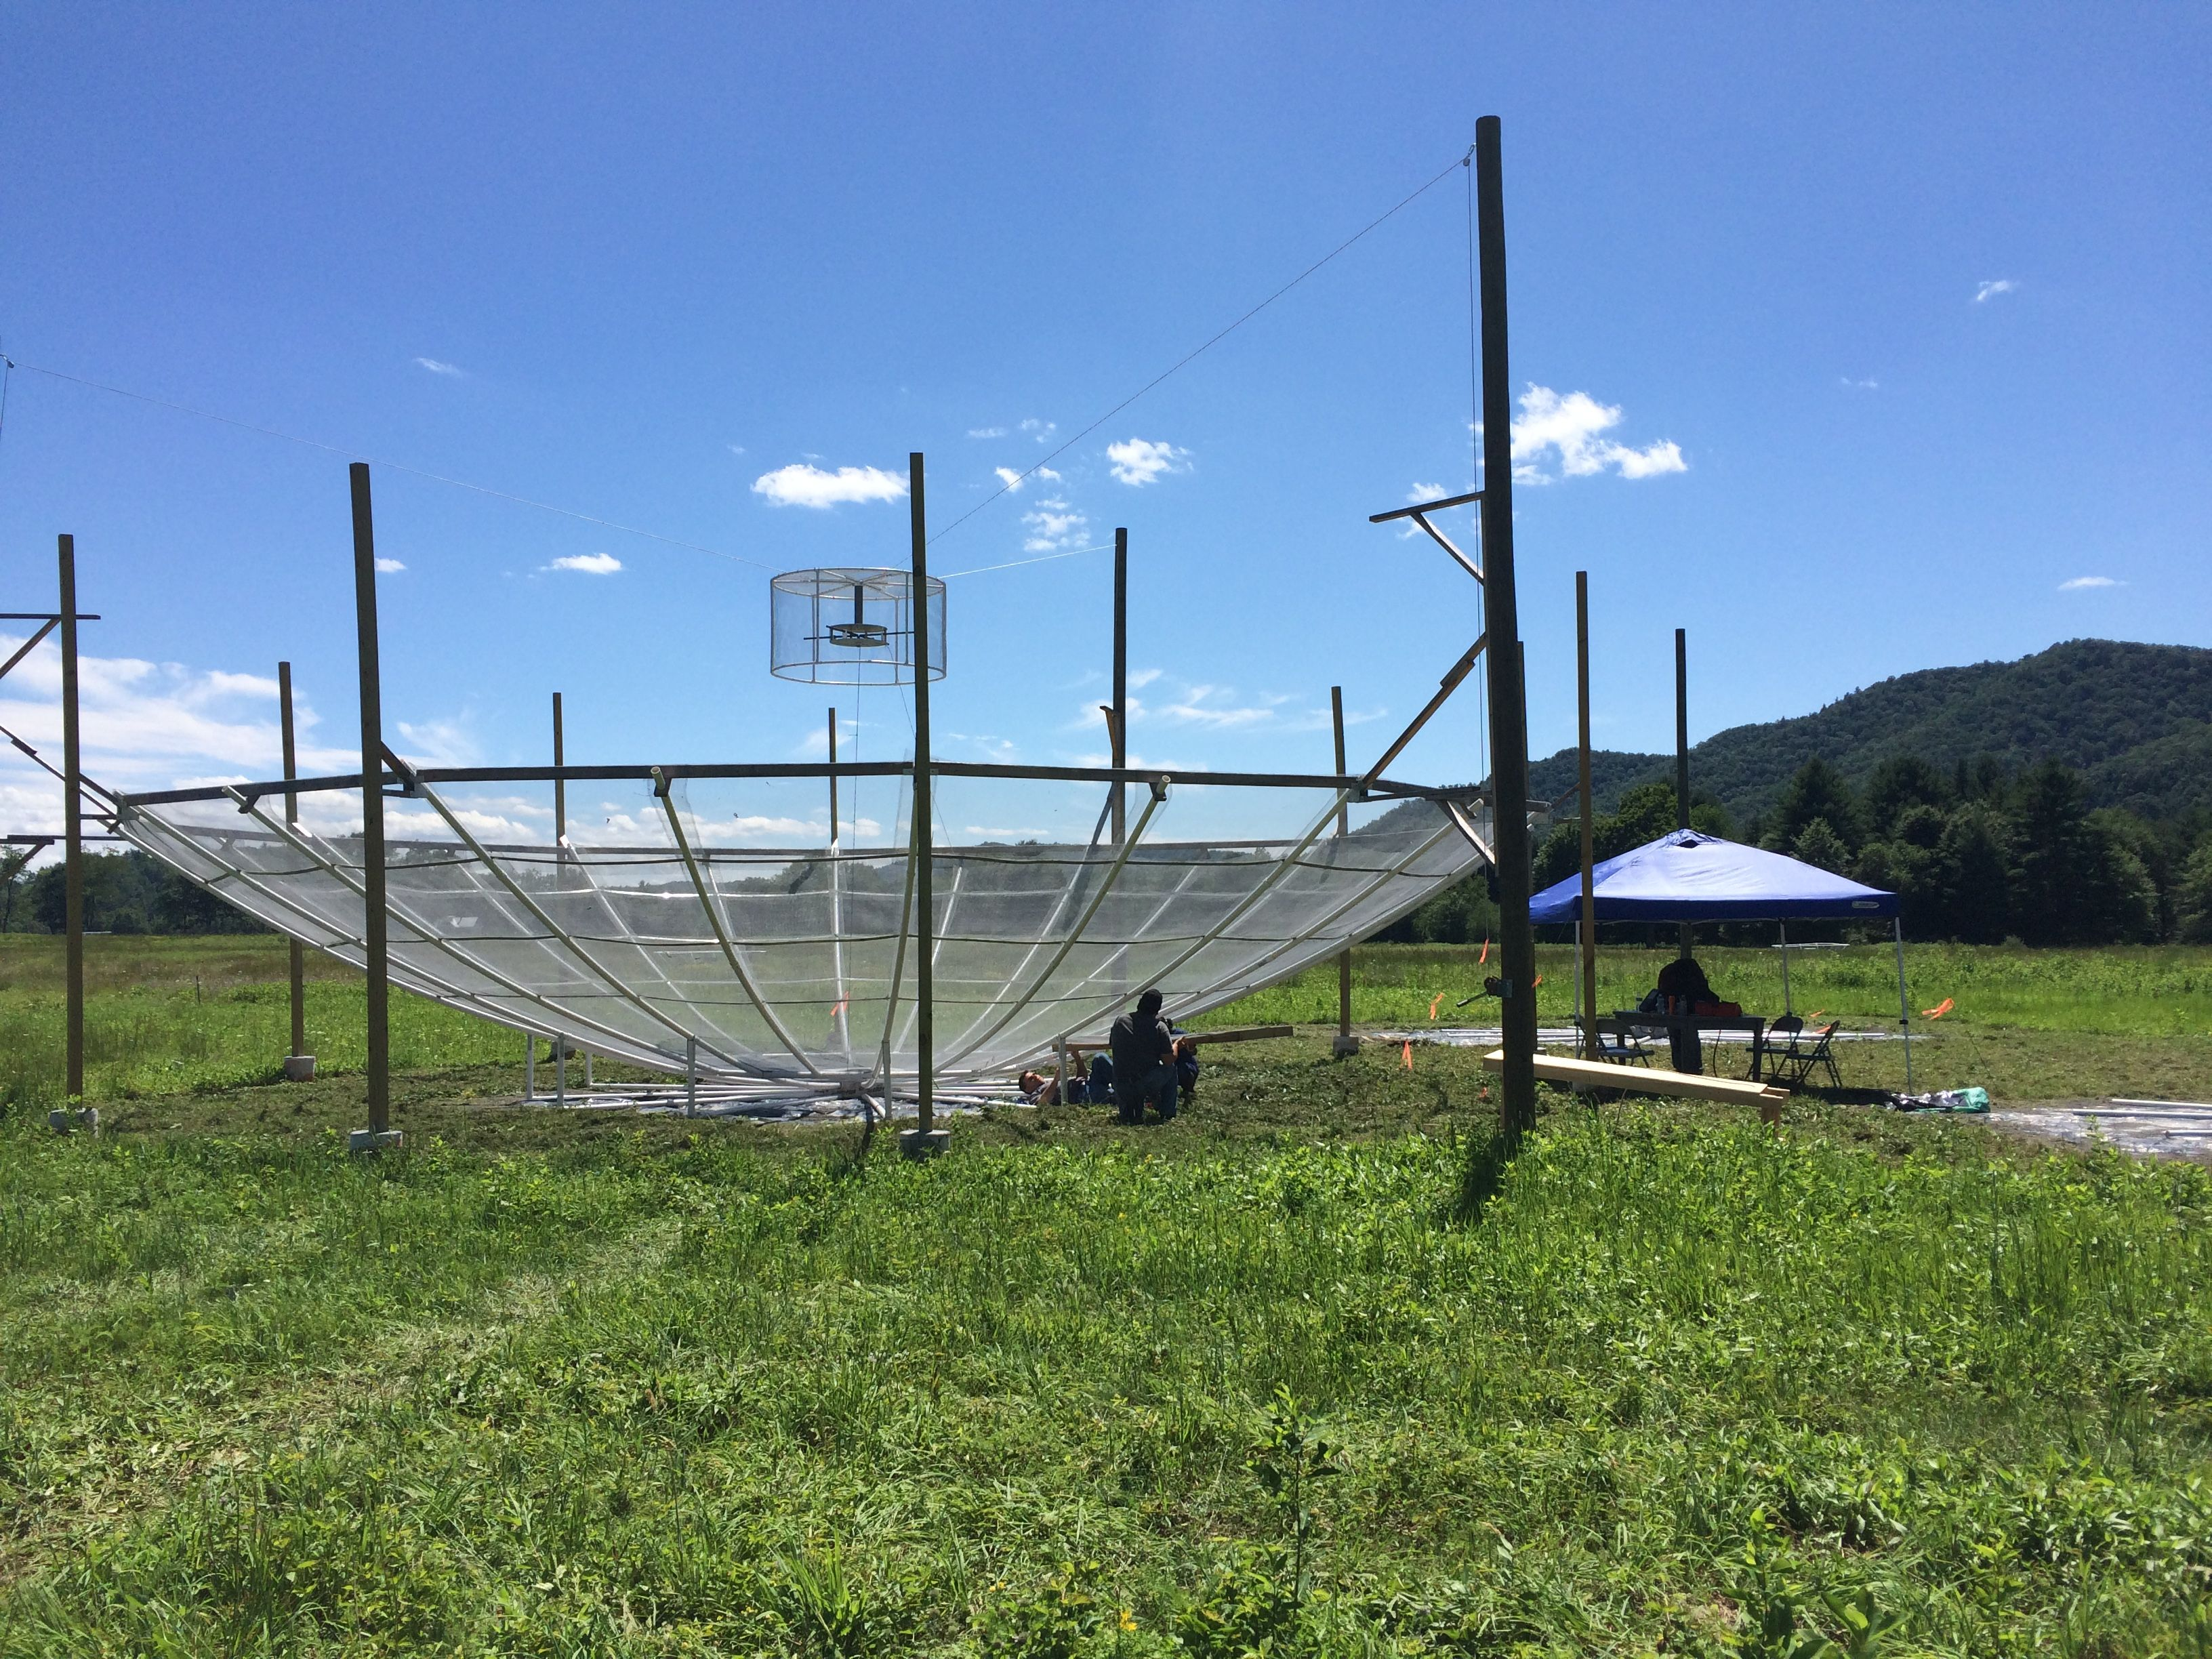
\includegraphics[trim={2cm 20cm 30cm 15cm},clip, totalheight=0.45\textheight]{heradish.jpg}
\caption{HERA dish and feed at the Green Bank NRAO site.}
\end{figure}

Reflectometry measurements were taken July 20-23, 2015 using a FieldFox Network Analyzer. A pulse was generated and sent through a cable (what type?) connecting to the feed. 

\section{Theory}

\section{Measurements}

\section{Discussion}

\section{Conclusion}


\end{document}
